% !TEX TS-program = xelatex
% !TEX encoding = UTF-8 Unicode
\documentclass[AutoFakeBold]{MyFormat}

\usepackage{listings}

\lstset{
 columns=fixed,       
 numbers=left,                                        % 在左侧显示行号
 numberstyle=\tiny\color{gray},                       % 设定行号格式
 frame=none,                                          % 不显示背景边框
 backgroundcolor=\color[RGB]{245,245,244},            % 设定背景颜色
 keywordstyle=\color[RGB]{40,40,255},                 % 设定关键字颜色
 numberstyle=\footnotesize\color{darkgray},           
 commentstyle=\it\color[RGB]{0,96,96},                % 设置代码注释的格式
 stringstyle=\rmfamily\slshape\color[RGB]{128,0,0},   % 设置字符串格式
 showstringspaces=false,                              % 不显示字符串中的空格
 language=c++,                                        % 设置语言
}

\begin{document}
%=====%
%
%封皮页填写内容
%
%=====%

% 标题样式 使用 \title{{}}; 使用时必须保证至少两个外侧括号
%  如: 短标题 \title{{第一行}},  
% 	      长标题 \title{{第一行}{第二行}}
%             超长标题\tiitle{{第一行}{...}{第N行}}

\title{{视频运动放大原理的学习}}
\entitle{{Learning Notes From 2022.06.08}}
\author{Sillin Ini\\Pinyi Huang}
\maketitle
\thispagestyle{empty}
\newpage

%生成目录
\tableofcontents
\thispagestyle{empty}
\newpage

%文章主体
\mainmatter




% =======正文从第一章开始
\setcounter{chapter}{0}

\chapter{关于学习过程中的疑问}


\section{关于训练和验证部分的代码}


\subsection{关于训练部分}
\par 在LOSO每一轮的训练中,其使用到的邻接矩阵似乎不同,\underline{{
为什么每一轮要使用不同的}}\\\underline{adj进行训练}?其代码如下:
\begin{lstlisting}
for idx in range(len(train_list)):
    npz_file = np.load(f"{args.npz_file}/{idx}.npz")
    adj_matrix = torch.FloatTensor(npz_file["adj_matrix"]).to(device)
    .............
    model = FMER(adj_matrix=adj_matrix,
                    num_classes=args.num_classes,
                    device=device).to(device)
\end{lstlisting}
\hspace*{\fill}
\par 在LOSO训练的每一轮15次epochs迭代中,其保存了效果最佳的参数,而在下一轮
训练时,则又重头开始训练,\underline{为什么不使用上一轮的最佳参数继续训练}?

\subsection{关于图像的预处理部分}
\par 关于图像为了输入MagNet所进行的预处理,为什么需要进行这些步骤?
可能因为我对MagNet的原理还没有了解很深,\underline{之后需要去了解具体细节吗}
?
\begin{lstlisting}
def unit_preprocessing(unit):
    unit = cv2.resize(unit ,(256, 256))
    unit = cv2.cvtColor(unit, cv2.COLOR_BGR2RGB)  # BGR To RGB
    unit = np.transpose(unit / 127.5 - 1.0, (2, 0, 1))
    unit = torch.FloatTensor(unit).unsqueeze(0)
    return unit

def unit_postprocessing(unit):
    unit = unit[0]
    # 将每个通道的图像归一化
    max_v = torch.amax(unit, dim=(1, 2), keepdim=True)
    min_v = torch.amin(unit, dim=(1, 2), keepdim=True)
    unit = (unit - min_v) / (max_v - min_v)
    unit = torch.mean(unit, dim=0).numpy()
    unit = cv2.resize(unit, (128, 128))
    return unit

def magnify_postprecessing(unit):
    unit = unit[0].permute(1, 2, 0).contiguous()
    unit = (unit + 1.0) * 127.5
    # 转变形状为[128, 128]
    unit = unit.numpy().astype(np.uint8)
    unit = cv2.cvtColor(unit, cv2.COLOR_RGB2GRAY)
    unit = cv2.resize(unit, (128, 128))
    return unit

# 具体实现部分
onset_frame = unit_preprocessing(cv2.imread(onset_file))
apex_frame = unit_preprocessing(cv2.imread(apex_file))
shape_representation, magnify = self.magnet(batch_A=onset_frame,
                                            batch_B=apex_frame,
                                            batch_C=None,
                                            batch_M=None,
                                            amp=amp,
                                            mode="evaluate")
magnify = magnify_postprecessing(magnify)
shape_representation = unit_postprocessing(shape_representation)
\end{lstlisting}



\chapter{关于MIT的欧拉影像放大算法\textit{Eulerian Video Magnification}}

\par 在这一节下,一共介绍有两种视角下的计算机影像放大方法。
\section{拉格朗日视角(\textit{Lagrangian Perspective})}
\par 在拉格朗日视角下,从跟踪图像中感兴趣的像素(粒子)的运动轨迹的角度分析。

\begin{itemize}
    \item 何为“变” —— 感兴趣的像素点随着时间的运动轨迹,
    这类像素点往往需要借助人工或其他先验知识来辅助确定;
    \item 放大“变” —— 将这些像素点的运动幅度加大。
\end{itemize}
\hspace*{\fill}
\par 在拉格朗日视角下,存在着以下几点不足:
\begin{itemize}
    \item 需要对粒子的运动轨迹进行精确的跟踪和估计,需要耗费较多的计算资源;
    \item 对粒子的跟踪是独立进行的,缺乏对整体图像的考虑,
    容易出现图像没有闭合,从而影响放大后的效果;
    \item 对目标物体动作的放大就是修改粒子的运动轨迹,
    由于粒子的位置发生了变化,还需要对粒子原先的位置进行背景填充,
    同样会增加算法的复杂度。
\end{itemize}



\section{欧拉视角(\textit{Eulerian Perspective})(
\textbf{\Large \underline{重点}})}
\par 欧拉视角将视角固定在一个地点,假定整幅图像都在变,
只是这些变化信号的频率、振幅等特性不同,
而我们所感兴趣的变化信号就身处其中。
\par 打个比方,同样是研究河水的流速,我们也可以坐在岸边,
观察河水经过一个固定的地方时的变化,
这个变化可能包含很多和水流本身无关的成分,
比如叶子掉下水面激起的涟漪,但我们只关注最能体现水流速的部分。
\begin{itemize}
    \item 何为“变” —— 整个场景都在变,而我们所感兴趣的变化信号藏在其中;
    \item 放大“变” —— 通过信号处理手段,将感兴趣的信号分离,并进行增强。\\
\end{itemize}


\par 欧拉影像放大技术的流程如下:
\begin{enumerate}
    \item 空间滤波:将视频序列进行金字塔多分辨率分解;
    \item 时域滤波:对每个尺度的图像进行时域带通滤波,
    得到感兴趣的若干频带(其中,对每一个像素点在时间轴上使用FFT快速傅里叶变换,
    将其转换至频域,之后使用特定的滤波器进行滤波;
    带通滤波的含义是:允许特定频段的波通过,
    同时屏蔽其他频段);
    \item 放大滤波结果:对每个频带的信号用泰勒级数来差分逼近,
    线性放大逼近的结果;
    \item 合成图像:合成经过放大后的图像。    
\end{enumerate}
\begin{figure}[!h]
    \centering
    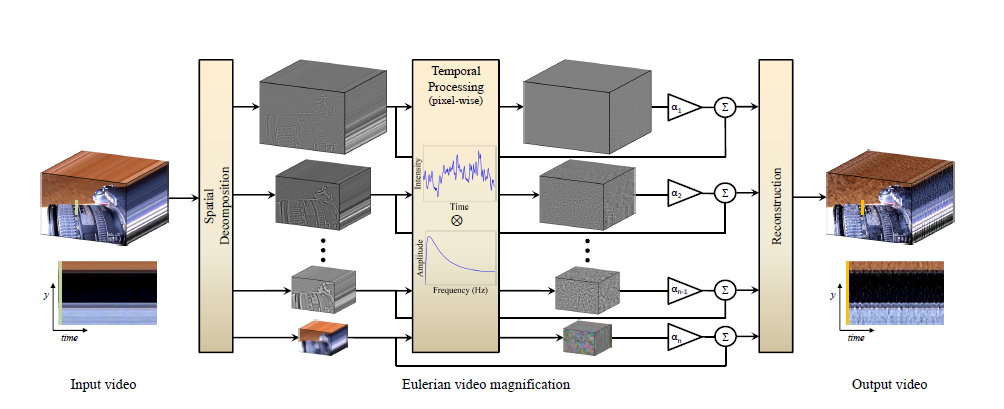
\includegraphics[width=\linewidth]
    {figures/2022.06.08/Eulerian Video mag.png}
    \caption{欧拉影像放大技术流程图}
\end{figure}

\par 这些技术通常包括三个阶段:将帧分解成运动表示、操纵该表示,以及将操纵
的表达重构为增强的帧。通常可以使用一阶泰勒展开式的空间分解,或使用复杂的
空间金字塔提取基于相位的表示。
\par 欧拉技术有助于揭示微妙的运动,但它们是手工设计的,没有考虑到许多问题,
如遮挡和大运动等。正因为如此,它们容易产生噪声,并且经常遭受过度模糊。

\par 但这种方法同样具有局限性:利用人工设计的过滤器来提取动作表示,
也许不是最佳的方法。


\section{基于神经网络的视频动作增强MagNet}
\par 在这个方法之前,所有的视频放大方法都饱受噪声和过度模糊等问题的困扰,
尤其是当放大倍数很大时。MagNet也属于欧拉方法,但其分解是直接从例子中学习的,
所以它具有更少的边缘伪影和更好的噪声特性。
\par 最近的技术通过使用光流或像素移位卷积核明确地移位像素,
这可以有高质量的结果。然而,当改变操纵因子的时候,这些技术通常需要重新训练。
\par 对于帧内插,MagNet的运动表示可以直接配置为不同的放大系数,不需要重新训练。
并且MagNet不使用任何明确的像素移动,这将需要一个可微分的双线性采样模块,
它可能不适合于子像素运动。
\par 对于帧外推最近有一系列工作直接合成 RGB 像素值来预测未来的动态视频帧,
但他们的结果往往很模糊。我们的工作专注于放大视频中的运动,
而不关心未来会发生什么。
\par 并且,MagNet在不使用时间滤波器的情况下,实现了与最新方法相似的效果。
\par MagNet直接从样例中使用CNN学习分解滤波器;
\par MagNet设计一个提取运动表示的网络,这样就可以通过简单地乘法,
并重建一个放大的帧。
\par MagNet神经网络主要由三个部分构成:
\begin{itemize}
    \item 空间分解滤波器Encoder:提取一个动作表示,类似于金字塔;
    \item 动作表示操作器Manipulator:接收这个动作表示,并操作它来增强动作,
    (通过乘以差异);
    \item 重构滤波器Decoder:将修改后的表示法重建为生成的运动放大帧。
\end{itemize}

\par 与欧拉视角的影像放大技术的各个部分的区别如下表所示:
\begin{center}
    \textbf{Table 1}~~神经网络模型训练参数表\\
    \setlength{\tabcolsep}{7mm}{
    \begin{tabular}{cccccc} \toprule
    使用的方法 & 欧拉视角增强 & MagNet\\ \hline
    空间分解 & 拉普拉斯金字塔 & 深度卷积层\\
    动作分离 & 时域带通滤波 & 减法或时域带通滤波\\
    去噪表示 & —— & 可训练卷积\\
    \bottomrule
    \end{tabular}}
\end{center}
\par Encoder和Decoder全是卷积的,这使得他们能在任意分辨率下起作用;并且使用
Residual Blocks残余模块生成高质量输出。为了节约内存空间和提升感受野,使用
Strided Convolution(即stride > 1)的卷积进行下采样;通过使用一个卷积层跟着
一个最近临域上采样,来避免棋盘状伪影。
\par 经过测试,Encoder中使用3个$3\times 3$残余模块和Decoder中使用9个
残余模块产生较好的效果。


\chapter{关于FGRMER模型的训练、验证部分代码}
\section{train.py}
\par 这部分代码用于实现模型的训练和验证。在训练部分采用了LOSO
(\textit{Leave One Subject Out},留一交叉验证)方法;而验证部分则是
一次对所有留下的Subject样本进行验证。

\par 在这一部分中,一共定义了三个函数,分别为:
\begin{itemize}
    \item LOSO\_train:用于实现留一交叉验证过程的函数;
    \item train:用于实现LOSO每一趟过程中的训练过程的函数;
    \item evaluate:用于实现每趟留一后,其余所有样本的识别准确率测试的函数。
\end{itemize}
\par 接下来对每个函数的细节进行剖析学习。


\subsection{LOSO\_train}
\par 其大致的步骤如下:
\begin{enumerate}
    \item 根据LOSO原则,生成一个train\_list和test\_list:这两个变量都是列表
    的形式,但其列表的每个元素都是一个pandas.DataFrame变量,列表的长度
    即为Subjects的数量27;
    \item 根据每个元素的下标,选取相应的adj\_file作为参数,构建Model;
    \item 使用交叉熵CrossEntropyLoss作为Criterion,Adam作为优化器,调用
    train函数进行训练;
    \item 训练完成后,在测试集上进行测试。将每次测试的准确率和F1-Score累加,
    最后取平均,由此查看模型的整体效果。
    并将每轮LOSO的结果写入一个log日志文件中。
\end{enumerate}


\subsection{train}
\par 在这一部分进行模型的训练,使用Criterion求loss,并根据反向传播,利用选择
的Adam优化器进行优化。
\par 对每一轮LOSO,train函数接收一个epochs参数,即训练轮数。在每一轮的训练
中,若模型准确率大于之前的最大准确率,就将该参数进行保存。
\par 在LOSO进行完一轮时,就实现了将最佳参数保存的效果。


\subsection{evaluate}
\par 在这一节中,使用了model.eval()的验证模式,同时还使用了torch.no\_grad
()来防止模型参数的改变。
\par 之后就是使用本轮LOSO中最佳的模型参数,来对测试集进行验证,分别求出了
准确率和F1-Score,并返回值。


\section{read\_file.py}
\par 在这个文件中,实现了对csv文件的读取和返回操作。返回了一个pd.DataFrame
变量,和一个label\_mapping,即{情绪分类:序号}的字典类型。
\par 值得一提的是,在label\_mapping变量生成的过程中,其是根据data.loc[:, 
"Estimated Emotion"]来获取数据的,即仅获取了这一列中的每一行。同时为了防止
字典中出现重复的情绪,其还使用了np.unique函数,在去重的同时还进行了排序。

\section{dataloader.py}
\par 在这个文件中,定义了两个函数:
\begin{itemize}
    \item get\_loader:实现了对自定义的DataLoader的返回。由于DataLoader的
    生成过程分为两步:第一步是写一个继承自torch.utils.data.Dataset类的自定义
    Dataset类;第二步是构造一个Dataloader对象。在这一个函数中,调用了其他
    文件中的自定义Dataset类,并生成了DataLoader对象,实现了返回。
    \item LOSO\_sequence\_generate:通过留一样本交叉验证LOSO方法,生成了
    一个train\_list和一个test\_list,两个列表的长度均为Subjects的数量。\\
    这个函数写的是真妙!\textbf{\Large \underline{反复学习!!}}
\end{itemize}


\section{dataset.py}
\par 在这个文件中,实现了一个自定义的Dataset类,用于构造DataLoader,以供
后续进行训练和验证。在这个部分,其对原始的图像进行了一系列的预处理,并在get\_
item方法中实现了这一系列操作。
\par 简单来说,其主要实现了以下几个步骤:
\begin{itemize}
    \item 输入一个item,通过item获取该表情的label标签;
    \item 读取一个Onset Frame图像和一个Apex Frame图像,首先进行预处理:
    转换图像的通道,并对每个通道进行归一化操作,使每个通道中的像素值映射在
    [-1, 1]之间。
    \item 随机选择一个放大倍数,并通过预训练好的MagNet模型进行输出,即得到
    一个形状表示shape\_representation和放大后的图像magnify。
    \item 将形状表示进行归一化操作,将像素值映射到[0, 1]之间,并将各个维度
    的像素值求平均,最后转变为$128\times 128$的图像。
    \item 放大后的图像magnify则将像素值从[-1, 1]区间映射回[0, 255]区间。
    并将其转化为灰度图像,将其形状变为[128, 128]。
    \item 最后,在magnify图像中获取人脸的特征点的坐标,在
    shape\_representation中获取30个patches,并于标签一起返回。
\end{itemize}








\end{document}